\documentclass{aip-cp}

\usepackage[numbers]{natbib}
\usepackage{rotating}
\usepackage{graphicx}
\usepackage[dvipsnames]{xcolor}
\usepackage{url}

\newif\iffinal
% Un-comment this line to see proposal without comments
%\finaltrue

\iffinal
    \newcommand\ian[1]{}
\else
    \newcommand\ian[1]{{\color{red}[Ian: #1]}}
\fi


% Document starts
\begin{document}

% Title portion
\title{Data Automation at Light Sources:\\Experiments and Lessons Learned\ian{more exciting title needed}}

\author[aff1,aff2]{Author's Name\corref{cor1}}
%\eaddress[url]{address@domain1.edu}
\author[aff2]{Author's Name}
%\eaddress{anotherauthor@thisaddress.yyy}

\affil[aff1]{Data Science and Learning Division, Argonne National Laboratory, Argonne IL 60439, USA.}
\affil[aff2]{Department of Computer Science, University of Chicago, Chicago IL 60637, USA.}
%\affil[aff3]{You would list an author's second affiliation here.}
\corresp[cor1]{Corresponding author: foster@anl.gov}
%\authornote[note1]{This is an example of first authornote.}
%\authornote[note2]{This is an example of second authornote.}

\maketitle


\begin{abstract}
%The AIP Proceedings article template has many predefined paragraph styles for you to use/apply as you write your paper. To format your abstract, use the \LaTeX template style: {\itshape Abstract.} Each paper must include an abstract. Begin the abstract with the word ``Abstract'' followed by a period in bold font, and then continue with a normal 9 point font.
Rapidly growing data volumes at light sources demand increasingly automated data collection, distribution, and analysis processes, in order to enable new scientific discoveries while not overwhelming finite human capabilities. I present here three projects that use cloud-hosted data automation and enrichment services, institutional computing resources, and high- performance computing facilities to provide cost-effective, scalable, and reliable implementations of such processes. In the first, Globus cloud-hosted data automation services are used to implement data capture, distribution, and analysis workflows for Advanced Photon Source and Advanced Light Source beamlines, leveraging institutional storage and computing. In the second, such services are combined with cloud-hosted data indexing and institutional storage to create a collaborative data publication, indexing, and discovery service, the Materials Data Facility (MDF), built to support a host of informatics applications in materials science. The third integrates components of the previous two projects with machine learning capabilities provided by the Deep Learning Hub (DLHub) to enable on-demand access to machine learning models from light source data capture and analysis workflows, and provides simplified interfaces to train new models on data from sources such as MDF on leadership scale computing resources. I draw conclusions about best practices for building next-generation data automation systems for future light sources.
\end{abstract}

\ian{Potential authors: Tekin Bicer, Ben Blaiszik, Kyle Chard, Ryan Chard, Logan Ward, Justin Wozniak, ...}


% Head 1
\section{INTRODUCTION}

Fourth-generation light sources such as the Advanced Photon Source Upgrade (APS-U)~\cite{APSU} will offer exciting new
scientific communities to the thousands of scientists who use their many beamlines annually.
They also pose major data and computation challenges, for at least four reasons.
First, they will generate massive data. 
For example, x-ray photon correlation spectroscopy can already generate 2MB images at 3,000 Hz,
for a data rate of 6 GB/s, comparable to that of the Large Hadron Collider~\cite{lhcrate}.
With APS-U, this data rate is expected to increase by 2--3 orders of magnitude.
Second, experiments will increasingly generate complex multi-modal data that needs advanced computing
for interpretation, such as ptychography combined with 
elemental mapping and visual images as a function of reaction conditions.
Third, it will become increasingly feasible to use advanced theory and modeling to fit and co-optimize 
model and experiment, so that 
Fourth, as synchrotron light source mature as instrucments, they increasingly serve more and different users,
many with limited or no experience with light sources. 
Automation is important for such users~\cite{hiraki2008high,toby2009management}.


Transition from artisanal/cottage industry to automated. Onsite not offsite. Capture data. Advanced analyses.

APS~\cite{toby2015practices}

References: MDF~\cite{MDF2016}, networking materials data~\cite{foster2015networking}, Justin~\cite{wozniak2015big}.


\section{DATA AUTOMATION}

\ian{Big picture thoughts I guess.}

Figures from my 

Choose next experiment.

 
\ian{Next text and Figure~\ref{fig:diffuse} are from~\cite{foster2015networking}. Need to be rewritten.}

As shown in Figure~\ref{fig:diffuse}, the resulting research process can involve a wide variety of interactions among experiment, computation, and human expertise for different purposes and at multiple timescales. 
On the right, we show diffuse scattering data being gathered for specific materials, with high-performance computing required for data analysis in order to provide timely feedback to experimenters. 
On the left, 
many simulations of potential structures are performed, using for example ab initio electronic structure codes, 
and potentially refined via evolutionary optimization, 
to create simulated diffuse scattering output that can be compared with experimental data. 
Ultimately, we want both experimental and simulation data to feed into an evolving knowledge base that can thenplay an important role in guiding current and future research. 
We also note that human collaboration and guidance is important at many points and scales, from direct steering of experiments to the choice of the next experiment and simulation 


\begin{figure}[h]
  \centerline{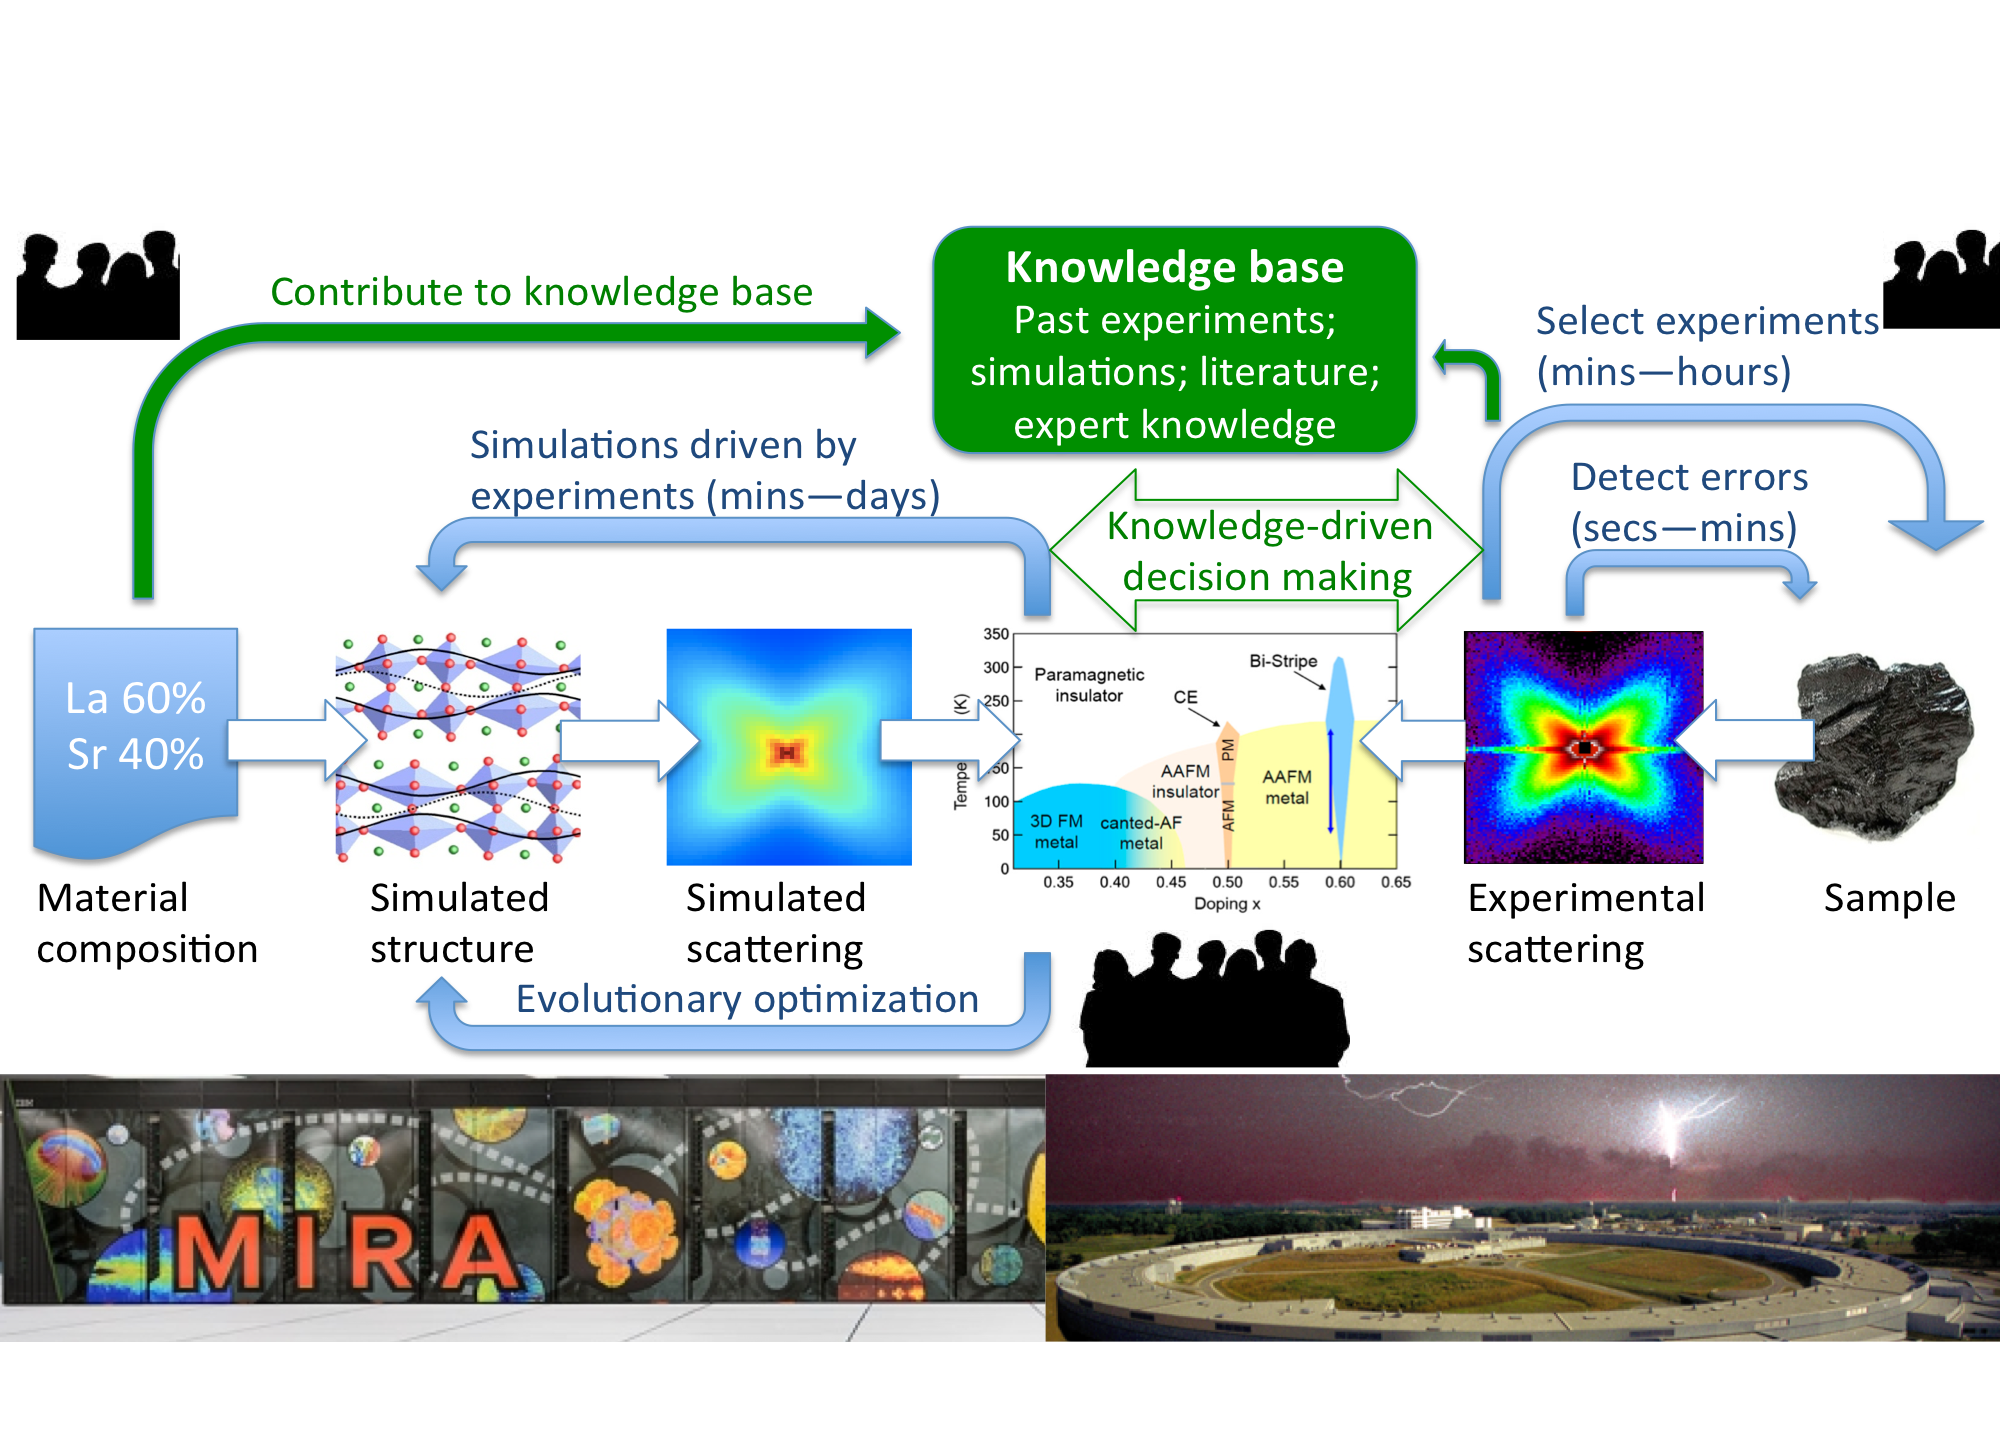
\includegraphics[width=6in,trim=0 2.6in 0 1.5in,clip]{Figs/diffuse.png}}
  \caption{Activities involved in a diffuse scattering experiment. 
  Acceleration and even automation of these various end-to-end processes, plus the creation of powerful knowledge base and simulation capabilities, can create a ``discovery engine'' for materials science research. 
  Note the publication phase by which data is contributed to the growing knowledge base.\label{fig:diffuse}}
\end{figure}


We first experimented with online analysis of APS in the late 1990s, 
when we coupled 
computing microtomography~\cite{wang1999quasi,wang2001high} and crystallographic~\cite{von2000using}
experiments to remote computers.
In one memorable demonstration in 1998, we piped microtomography data from APS beamline 2-BM to a 96-node SGI Origin parallel computer 
at Argonne for incremental reconstruction via filtered backprojection as an experiment was proceeding,
and then streamed visualization data to the Supercomputing conference (SC'98) in Orlando, Florida, 
for interactive analysis: see Figure~\ref{fig:sc98}. 
As we noted at the time, 
``the data rates and compute power required ... are prodigious, easily reaching one gigabit per second and a teraflop per second [respectively]"~\cite{von2000real}---numbers that are dwarfed by today's requirements. 

\begin{figure}[h]
  \centerline{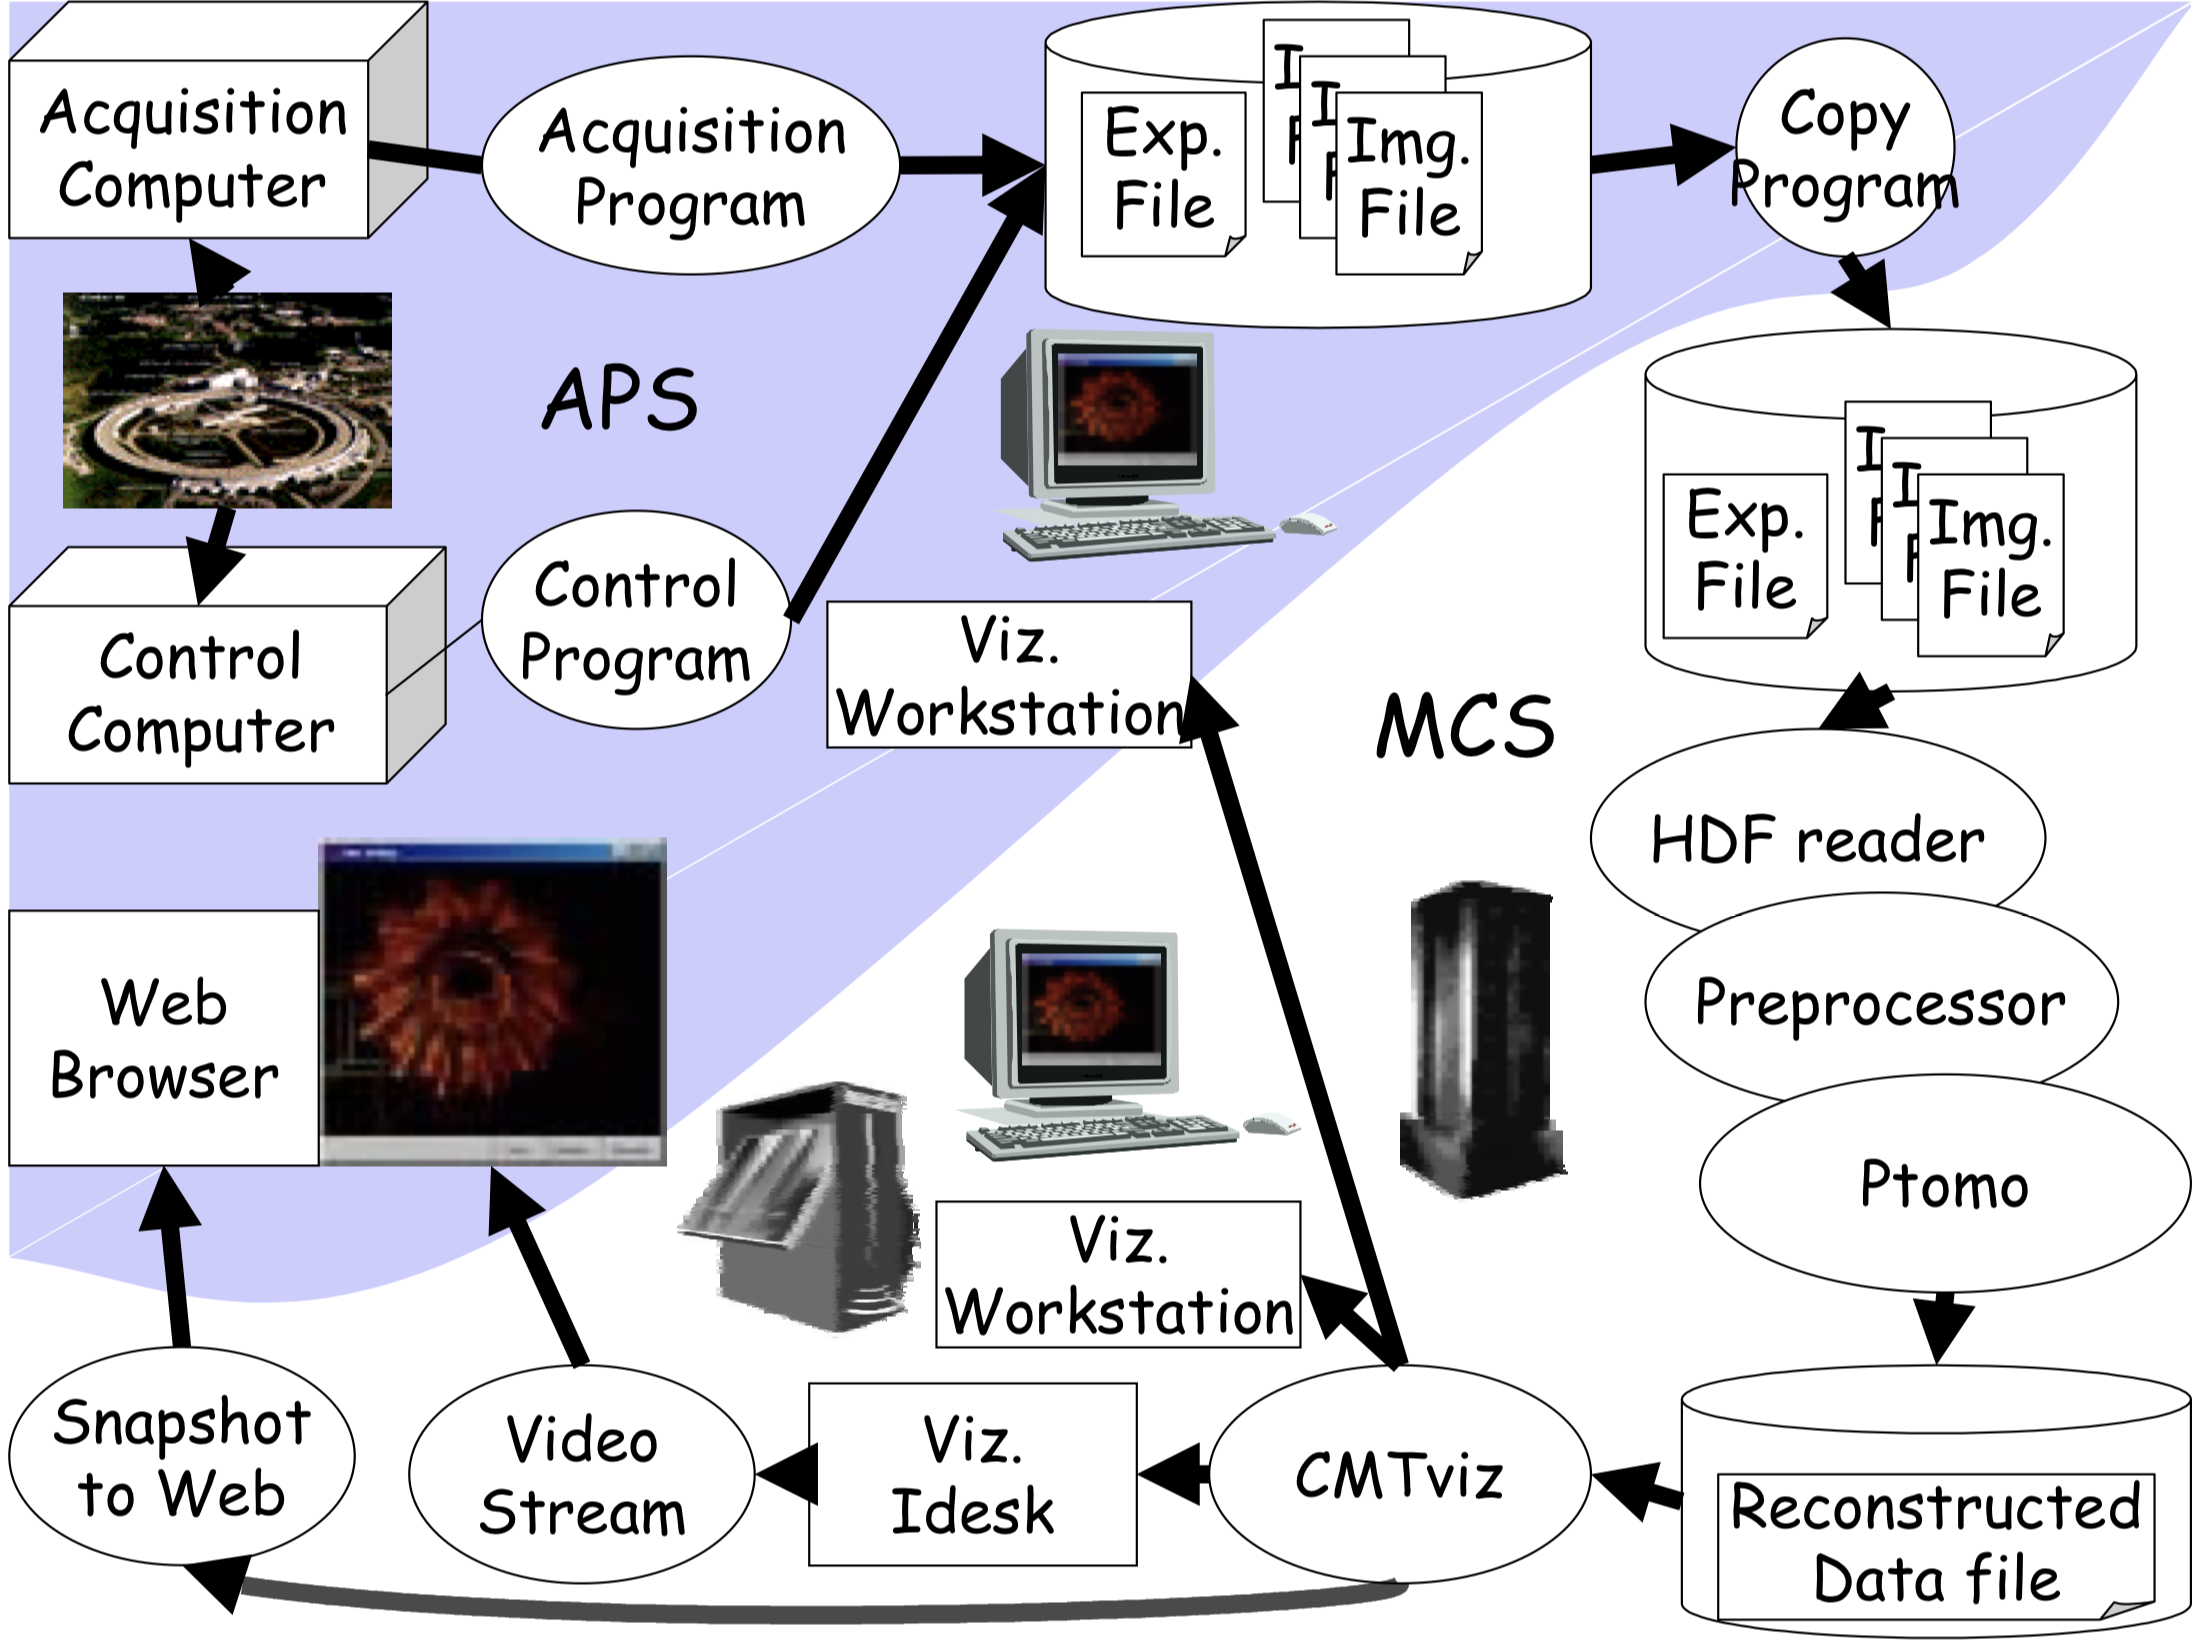
\includegraphics[width=4in]{Figs/APS-Fig.png}}
  \caption{The processing pipeline used in the SC'98 demonstration~\cite{von2000real}. Data collected at the APS 
  where passed to supercomputer in Argonne's Mathematics and Computer Science (MCS) division for
  incremental reconstruction and visualization, and results dispatched as a stereoscopic
  video stream to a remote virtual reality displays at APS and in Orlando.\label{fig:sc98}}
\end{figure}

\section{DATA ACQUISITION AND DISTRIBUTION}

Sharma, Wozniak, and others developed an online analysis pipeline for high energy diffraction microscopy
experiments 

HEDM work to be described somewhere~\cite{park2015high}.

\cite{delageniere2011ispyb}: 
ISPyB: An information management system for synchrotron macromolecular crystallography

pipeline~\cite{wozniak2015big}


\ian{Petrel should get a mention.}



\section{MDF: DATA PUBLICATION AND INDEXING}

TBD.


\section{DLHUB: AUTOMATED ANALYSIS AND LEARNING}

TBD.

DLHub is a project to promote, simplify, and speed the widespread adoption and usage of machine learning and deep learning techniques by researchers in disciplines ranging from materials science to chemistry, physics, cosmology, and biology. The co-emergence of large amounts of available datasets, movement towards cohesive data services, and new machine learning and, especially, deep learning (ML/DL) capabilities, creates a unique opportunity to leverage and integrate these data streams to allow for ML/DL techniques to guide and, indeed, lead discovery efforts.
 
Thus, we are developing DLHub (Fig. 1), a self-service platform for publishing, applying, and creating new ML/DL models. DLHub will provide: 1) publication capabilities to make models more discoverable, citable, and reusable; 2) the ability to easily run or test existing models; and 3) links to the data and computing infrastructure to re-train models for new applications. Users will benefit from DLHub in many ways. Data scientists can publish their models (i.e., architectures and weights) and methods. Materials scientists can apply existing models to new data with ease (e.g., by querying a prediction API for a deployed mode) and create new models with state-of-the-art techniques. Together, these capabilities will lower barriers to employing ML/DL, making it easier for researchers to benefit from advances in ML/DL technologies. 


Parallel tomo~\cite{Bicer_Europar15}. Real-time steering~\cite{bicer2017real}.

\section{RELATED WORK}

Coles et al.~\cite{coles2005ecses,coles2006science} developed an automated small molecule crystallography service that automated the
end-to-end-flow from sample receipt to results dissemination.

PNNL work~\cite{thomas2015towards}. Helmholtz work~\cite{gehrke2015high}. BNL work~\cite{deslippe2014workflow}.


\section{SUMMARY}









\section{ACKNOWLEDGMENTS}

This work was supported in part by DOE contract DE-AC02-06CH11357 and by award 70NANB14H012 from the U.S.\  Department of Commerce, National Institute of Standards and Technology as part of the Center for Hierarchical Materials Design (CHiMaD)..
We are grateful to colleagues at the Argonne Photon Source and other synchrotron light sources
for many helpful discussions.

% References

\nocite{*}
\bibliographystyle{aipnum-cp}%
\bibliography{Bibs/refs}%


\end{document}
